\section{Método de Newton}
%\index{Método de Newton}

\subsection{Características}

\begin{itemize}
 \item Necessita uma aproximação inicial da raíz desejada.
 \item Usa a reta tangente calculada analiticamente.
 \item Pode ser aplicado para o cálculo de raízes complexas.
 \item Derivado a partir da expansão de Taylor.
\end{itemize}

\subsection{Descrição do Método}

\begin{equation}
 \label{eq:newton1}
 f(x) = 0 = f(x_{0} + f'(x_{0}) \ast (x - x_{0})) + O(h^{2})
\end{equation}

\[
 \displaystyle \left( \frac{f^{(n)}(x_{0})}{n!} \ast h^{n} \right)
\]

onde $h = x - x_{0}$.

Desprezando $O(h^{2})$ e resolvendo \ref{eq:newton1}, temos:

\begin{equation}
 \label{eq:newton2}
 x = x_{0} - \frac{f(x_{0})}{f'(x_{0})}
\end{equation}

Devido ao erro de truncamento, $x$ encontrado em \ref{eq:newton2} não é a solução de \ref{eq:newton1}, mas é uma melhor aproximação do que $x_{0}$.

\begin{figure}[htb]
  %\index{figura da posição falsa modificado}%
  \setlength{\abovecaptionskip}{20pt}
  %%% o valor default de \abovecaptionskip definido para a classe
  %%% article e de 10pt.
  \centering
  %%% VIDE ABAIXO COMENTARIO SOBRE USO DE DIRETORIOS NO PATHNAME
  %%% DOS ARQUIVOS INCLUIDOS.
  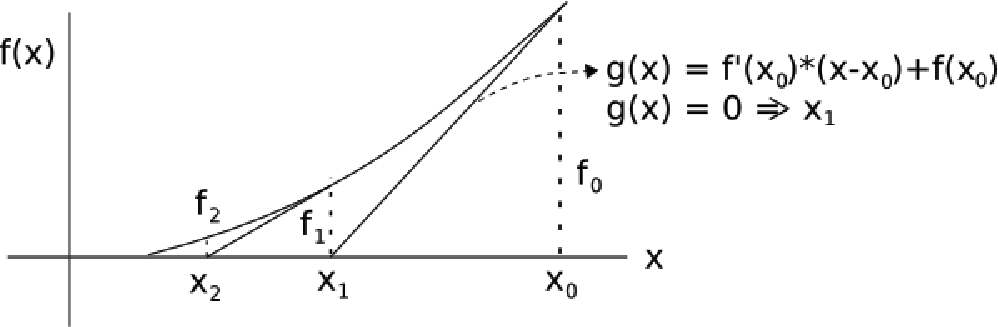
\includegraphics[scale=0.8]{capitulos/capitulo1/figuras/newton1-eps-converted-to.pdf}
  \caption{Ilustração para o método de Newton.}
  \label{fig:newton1}
\end{figure}

\[\displaystyle x_{i} = x_{i-1} - \frac{f(x_{i-1})}{f'(x_{i-1})}\]

\textbf{Notas:}

\begin{enumerar}
 \item O cálculo de $f'(x)$ pode ser difícil ou impossível. Nesses casos utiliza-se aproximação por diferenças finitas:

 \begin{itemize}
  \item \textit{Forward} $\displaystyle \rightarrow f'(x_{i-1}) \approx \frac{f(x_{i-1} + h) - f(x_{i-1})}{h} \, $ onde $h$ é um valor pequeno.

  \item \textit{Backward} $\displaystyle \rightarrow f'(x_{i-1}) \approx \frac{f(x_{i-1}) - f(x_{i-1} - h)}{h}$
 \end{itemize}

 \item Pequenos erros no cálculo de $f'(x_{i-1})$ não afetam muito a taxa de convergência.

 \item Se $f(x)$ não tem ponto de singularidade na vizinhança da raiz, as duas aproximações por diferenças finitas funcionam bem.

 \item Este método é de primeira ordem porque utiliza a primeira derivada.

 \item Métodos de segunda ordem teriam uma convergência mais rápida, mas o cálculo de derivada segunda, geralmente, elimina a vantagem sobre o método de primeira ordem.

\end{enumerar}

\begin{example}
 Derive um esquema iterativo baseado no método de Newton para encontrar a raiz cúbica de um número. Encontre a raiz de 155.

 \textbf{Solução:}

\[
\sqrt[3]{a} = x \Rightarrow x^{3} = a \Rightarrow f(x) = x^{3} - a
\]
 
Aplique o método de Newton

\[
 x_{n+1} = x_{n} - \frac{f(x_{n})}{f'(x_{n})} = x_{n} - \frac{x_{n}^{3} - a}{3 \ast x_{n}^{2}}
\]

\[
 x_{n+1} = \frac{2}{3} \ast x_{n} + \frac{a}{3 \ast x_{n}^{2}}
\]

Cálculo de $\sqrt[3]{155} \Rightarrow a = 155$.

\begin{enumerar}
\item Estimativa inicial $x_{0} = 5$:

\begin{table}[htp]
\footnotesize
	\centering
		
		\begin{tabular}{|c|c|c|}
		\hline		
		\textbf{$n$} & \textbf{$x$} & \textbf{$\displaystyle | x_{n+1} - x_{n} |$}\\
		\hline \hline 
		0 & 5 & -\\
		\hline 
		1 & 5.4 & 0.4\\
		\hline 
		2 & 5.371834 & 0.028\\
		\hline 
		3 & \underline{5.371685} & 0.00014\\
		\hline
		\end{tabular}
	%\caption{Iterações do método da bisseção}
	\caption{Exemplo de iterações do método de Newton para $x_{0} = 5$.}
	\label{tab:newton1}
\end{table}

\item Estimativa inicial $x_{0} = 10$:

\begin{table}[htp]
\footnotesize
	\centering
		
		\begin{tabular}{|c|c|c|}
		\hline		
		\textbf{$n$} & \textbf{$x$} & \textbf{$\displaystyle | x_{n+1} - x_{n} |$}\\
		\hline \hline 
		0 & 10 & -\\
		\hline 
		1 & 7.183334 & 2.816666\\
		\hline 
		2 & 5.790176 & 1.393158\\
		\hline
		3 & 5.401203 & 0.388973\\
		\hline
		4 & 5.371847 & 0.029383\\
		\hline
		5 & \underline{5.371686} & 0.000161\\
		\hline
		\end{tabular}
	%\caption{Iterações do método da bisseção}
	\caption{Exemplo de iterações do método de Newton para $x_{0} = 10$.}
	\label{tab:newton2}
\end{table}

\end{enumerar}

\end{example}

\begin{example}
\label{ex:newton1}

Encontre a primeira raiz positiva de $y = \tan(x) - 0.5 \ast x$ pelo método de Newton.

\textbf{Solução:}

\[
 y' = \frac{1}{\cos^{2}(x)} - 0.5 = \tan^{2}(x) + 0.5
\]

\[
 x_{n+1} = x_{n} - \frac{\tan(x_{n}) - 0.5 \ast x_{n}}{\tan^{2}(x_{n}) + 0.5}
\]

\begin{figure}[htb]
  %\index{figura da posição falsa modificado}%
  \setlength{\abovecaptionskip}{20pt}
  %%% o valor default de \abovecaptionskip definido para a classe
  %%% article e de 10pt.
  \centering
  %%% VIDE ABAIXO COMENTARIO SOBRE USO DE DIRETORIOS NO PATHNAME
  %%% DOS ARQUIVOS INCLUIDOS.
  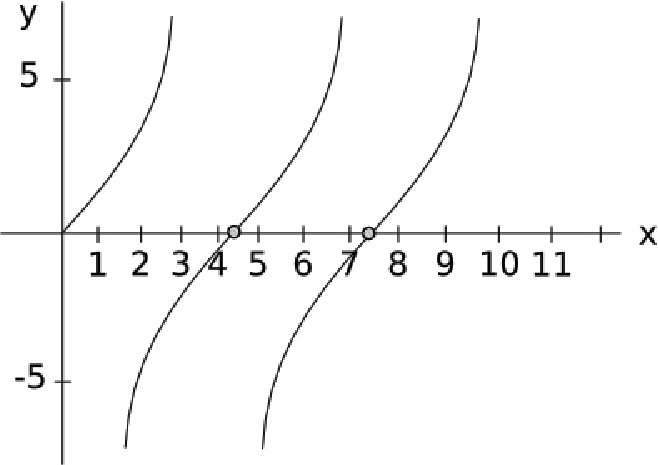
\includegraphics[scale=0.8]{capitulos/capitulo1/figuras/newton2-eps-converted-to.pdf}
  \caption{Ilustração para o método de Newton.}
  \label{fig:newton2}
\end{figure}

\begin{enumerar}
\item $\xi = 0.0001$

\item $x_{0} = 4$

\begin{table}[htp]
\footnotesize
	\centering		
		\begin{tabular}{|c|c|c|}
		\hline		
		\textbf{$n$} & \textbf{$x$} & \textbf{$\displaystyle | x_{n+1} - x_{n} |$}\\
		\hline \hline 
		0 & 4 & -\\
		\hline 
		1 & 4.458280 & 0.458280\\
		\hline 
		2 & 4.352068 & 0.106212\\
		\hline
		3 & 4.288511 & 0.033557\\
		\hline
		4 & 4.275191 & 0.013320\\
		\hline
		5 & 4.274782 & 0.000409\\
		\hline
		6 & \underline{4.244782} & 0.000000\\
		\hline
		\end{tabular}
	%\caption{Iterações do método da bisseção}
	\caption{Iterações do método de Newton para $x_{0} = 4$.}
	\label{tab:newton3}
\end{table}

\item $\xi = 0.0001$

$x_{0} = 3.6$

\begin{table}[htp]
\footnotesize
	\centering		
		\begin{tabular}{|c|c|c|}
		\hline		
		\textbf{$n$} & \textbf{$x$} & \textbf{$\displaystyle | x_{n+1} - x_{n} |$}\\
		\hline \hline 
		0 & 3.6 & -\\
		\hline 
		1 & 5.358891 & 1.758891\\
		\hline 
		2 & 7.131396 & 1.772505\\
		\hline
		3 & 8.494651 & 1.363255\\
		\hline
		4 & 10.92057 & 2.425919\\
		\hline
		5 & 10.87581 & 0.04476\\
		\hline
		6 & 10.83419 & 0.04162\\
		\hline
		7 & 10.81511 & 0.01908\\
		\hline
		8 & 10.81269 & 0.00242\\
		\hline
		9 & \underline{10.81267} & 0.00002\\
		\hline
		\end{tabular}
	%\caption{Iterações do método da bisseção}
	\caption{Iterações do método de Newton para $x_{0} = 3.6$.}
	\label{tab:newton4}
\end{table}

\end{enumerar}

\end{example}

\noindent
\textbf{OBS:}

\begin{itemize}
 \item O m\'etodo necessita de uma boa estimativa inicial, caso contr\'ario a solu\'c\~ao iterativa pode divergir ou convergir para uma solu\'c\~ao iterativa irrelevante.

 \item A taxa de converg\^encia elevada \`a  medida que se aproxima da solu\'c\~ao iterativa.
\end{itemize}

Suponha que $x$ seja a solução.

\begin{description}
\item[] $f(x) = f(x_{i}) + f'(x_{i}) \ast \xi_{i} + \displaystyle \frac{1}{2} \ast f''(x_{i}) \ast \xi_{i}^{2} + ... = 0$

\item[] $f'(x_{i}) = - f'(x_{i}) \ast \xi_{i} - \displaystyle \frac{1}{2} \ast f''(x_{i}) \ast \xi_{i}^{2}$

\item[] Método de Newton $\displaystyle \Rightarrow x_{i+1} = x_{i} - \frac{f(x_{i})}{f'(x_{i})} $

\item[] $\displaystyle x - x_{i+1} = x - x_{i} + \frac{f(x_{i})}{f'(x_{i})} \Rightarrow$

\item[] $\displaystyle  \Rightarrow \xi_{i+1} = \xi_{i} - \frac{f'(x_{i}) \ast \xi_{i}}{f'(x_{i})} - \frac{f''(x_{i}) \ast \xi_{i}^{2}}{2 \ast f'(x_{i})} \Rightarrow$

\item[] $\displaystyle \Rightarrow \xi_{i+1} = - \frac{f''(x_{i})}{2 \ast f'(x_{i})} \ast \xi_{i}^{2}$

\item[] $\displaystyle \xi_{i+1} = - \xi_{i}^{2} \ast \frac{f''(x)}{2 \ast f'(x)}$

\end{description}